\documentclass[12pt]{article}
%\usepackage[utf8]{inputenc}
\usepackage[T1]{fontenc}
\usepackage{graphicx}
\usepackage{xcolor}
\usepackage{multirow,multicol}
\usepackage{rotating,colortbl}
%\usepackage[utf8x]{inputenc}
\usepackage{csquotes,xpatch}
\usepackage[backend=biber, style=apa]{biblatex}
\usepackage{tikz}
\usetikzlibrary{shapes.geometric, arrows}
%%novalidate

\usepackage{tikz}
\usepackage{calc}
\usepackage{booktabs}


% colors
\definecolor{color1}{HTML}{000060}
%\definecolor{color1}{HTML}{8C260F}
\definecolor{color2}{HTML}{333333}


% fonts
\usepackage{fontspec}
\defaultfontfeatures{Mapping=tex-text}
\setmainfont
[BoldFont=Lato-Bold.ttf,
ItalicFont=Lato-Italic.ttf,
BoldItalicFont=Lato-BoldItalic.ttf]
{Lato-Regular.ttf}
\newfontfamily\headingfont[ItalicFont=Lato-BlackItalic.ttf]{Lato-Black.ttf}
%%%

\usepackage{geometry}
\geometry{letterpaper,
hmargin=20mm,vmargin=20mm,
head=0ex,foot=3ex}

\linespread{1.3}

\usepackage[hang]{caption}
\DeclareCaptionFormat{upper}{#1#2\uppercase{#3}\par}
\captionsetup{labelfont={bf,color=color2},textfont={normalsize,color=color2},format = upper,figurename=FIGURE,tablename=TABLE}

%%% fancy sections
\usepackage{titlesec}
%\titleformat{\chapter}{\headingfont\LARGE\bfseries\scshape\color{color1}}{\thechapter}{1em}{}[\titlerule]
\titleformat{\section}{\color{color1}\headingfont\Large\bfseries\uppercase}{\thesection}{1em}{}[\titlerule]
\titleformat{\subsection}{\color{color1}\headingfont\large\bfseries\uppercase}{\thesubsection}{1em}{}
\titleformat{\subsubsection}{\color{color1}\headingfont\bfseries\uppercase}{\thesubsubsection}{1em}{}
%%%

% head and foot
\usepackage{fancyhdr}
\pagestyle{fancy}
\lhead{}
\chead{}
\makeatletter
\rhead{\color{color2}\@date}
\makeatother
\newlength{\myheight}
\lfoot{
\settoheight{\myheight}{\thepage}
\raisebox{-2ex-0.5\myheight}{
\includegraphics[height=4ex]{logo}}
}
\cfoot{\color{color2}Threat Assessment for Inchcape Shipping Services}
\rfoot{\color{color2}\thepage}
\renewcommand\headrulewidth{0pt}
\renewcommand\footrulewidth{0pt}

% custom titlepage
\makeatletter
\newcommand*\DefVar[1]{\@namedef{#1}##1{\global\@namedef{get#1}{##1}}}
\DefVar{summary}
\renewcommand{\maketitle}{
\begin{center}

\begin{tikzpicture}
    \node[draw=none,%color1,line width=0.4pt,
      fill=color1,
      inner sep = 10pt,
      text width=\textwidth-20pt,
      text centered
    ] {\color{white}\headingfont\bfseries\huge\@title};
\end{tikzpicture}

\includegraphics[width=\textwidth]{opening}\par
\headingfont\bfseries\Large\@author\par
\bigskip\medskip
{\color{color2}\normalfont\normalsize\textbf{Summary:}\\
\getsummary}
\end{center}
\clearpage
}
\makeatother
%%%

%%% fancy boxes
\usepackage{tcolorbox}
\usepackage{wrapfig}
\def\fullboxbegin{
\bigskip
\begin{tcolorbox}[colback=color1,colframe=color1,coltext=white,arc=0mm,boxrule=0pt]
}
\def\fullboxend{\end{tcolorbox}\medskip}
%
\def\leftboxbegin{
\begin{wrapfigure}{l}{0.5\textwidth}
\begin{tcolorbox}[colback=color1,colframe=color1,coltext=white,arc=0mm,boxrule=0pt]
}
\def\leftboxend{
\end{tcolorbox}
\end{wrapfigure}
}
%
\def\rightboxbegin{
\begin{wrapfigure}{r}{0.5\textwidth}
\begin{tcolorbox}[colback=color1,colframe=color1,coltext=white,arc=0mm,boxrule=0pt]
}
\def\rightboxend{
\end{tcolorbox}
\end{wrapfigure}
}
%
\newcounter{frames}
\def\frameboxbegin#1{
\bigskip
\refstepcounter{frames}
\begin{tcolorbox}[colback=white,colframe=color1,arc=0mm,title={\MakeUppercase{\textbf{Frame \arabic{frames}}: #1}}]
}
\def\frameboxend{
\end{tcolorbox}
}
%%%
\addbibresource{Threat Assessment.bib}
%\usepackage{lipsum}
\usepackage[hidelinks]{hyperref}
\usepackage{tikz}
\usepackage{xparse}

\newcounter{chatlinenum}

%% Adjust text width to suit
\tikzset{chatstyle/.style={text width=1.5in,rounded corners=2pt}}

%% Adjust width of minipage to suit, but greater than TikZ text width
\NewDocumentEnvironment{chat}{}{%
   \setcounter{chatlinenum}{0}
   \begin{minipage}{3.0in}
       \everypar={\chatline}
}{%
   \end{minipage}
}

\definecolor{mygreen}{HTML}{88EABB}

%% Alter colors to suit
\def\chatline#1\par{%
   \stepcounter{chatlinenum}%
   \noindent
   \ifodd\thechatlinenum
       \tikz[]{\node[fill=lightgray,chatstyle]{\strut#1\strut};}%
   \else
       \hfill
       \tikz[]{\node[fill=mygreen,chatstyle,align=right]{\strut#1\unskip\strut};}%
   \fi
   \par
   \smallskip
}

%% |=====8><-----| %% New solution:

%% Alter colors to suit
\begingroup
    \lccode`~=`\^^M
    \lowercase{%
\endgroup
    \def\newchatline#1~{%
        \stepcounter{chatlinenum}%
        \ifodd\thechatlinenum
            \tikz[]{\node[fill=lightgray,chatstyle]{\strut#1\strut};}%
        \else
            \hfill
            \tikz[]{\node[fill=mygreen,chatstyle,align=right]{\strut#1\strut};}%
        \fi
        ~
        \smallskip
    }%
}

\NewDocumentEnvironment{newchat}{}{%
    \setcounter{chatlinenum}{0}
    \begin{minipage}{3.0in}
        \obeylines
        \everypar={\newchatline}
}{%
    \end{minipage}
}
\hyphenation{Inchcape}
%\usepackage{float}
\setlength{\headheight}{15pt}
\let\footcite\footfullcite
%%%%%%%%%%%%%%%
% Title Page
\title{Threat Assessment for Inchcape Shipping Services}
\author{Joey Simone\\GMA420 - Cybersecurity}
\date{April 19th, 2024}
\summary{
At Inchcape, a breach could expose data for hundreds of ships and workers, a denial of service could slow or interrupt the flow of ships in and out of ports wherever the company operates. I recommend that you harden outside facing appliances, such as websites, maintain adequate security on the physical premises, invest in intrusion detection and prevention software, and most importantly: train \textbf{all personnel} to recognize the signs of Social Engineering and Phishing. 
}
%%%%%%%%%%%%%%%

\begin{document}
\maketitle

%\tableofcontents
%\clearpage

\section{Attack Surface}
\subsection{Target Overview}
Companies like Inchcape are at risk because of the utility that they provide to ships and shipping companies. They hire logistics professionals like Port Agents and Ship Managers to make the port call experience as seamless and painless as possible. As the local representative, they can book repairs, last mile logistics, chandling, bunkering, husbandry, and dry docking. They can handle some of the paperwork load and remittance banking on behalf of carriers, and their ship managers dynamically fill the needs of the ship and her crew. \footcite{noauthor_efficient_2022}
This close contact with ships at critical point in their careers, their port calls and their at-dock maintenance, means that hostile actors can have undue influence on the ecosystem of shipping by exerting control over a company like Inchcape. 

\section{Potential Vulnerabilities}
\subsection{Human Vulnerabilities} Like most jobs in the modern economy, all Shipping Service company employees are info-handlers. Employees' duties require exchanging calls, emails, files, and physically visiting locations. Some of the legitimate businesses and ships may have people without perfect grasp of the English Language, which is often a sign of a phishing attack. Agents masquerading as legitimate business contacts may interact with employees and launch Social Engineering attacks, asking questions they shouldn't to access confidential information. Ship agents have to respond to needs quickly; make contact and maintain relationships with ships, port authorities, and port businesses; and handle significant quantities of private or privileged data. These factors may put them at risk of being targeted by threat actors. A ship manager with a TWIC to enter a port may be piggybacked\footnote{piggybacking is when an unauthorized person follows an authorized person into a restricted area.}. Any of the various external emails that an employee comes across may be a phishing email, or the attachments may be concealing malware. The attack surface is every method of communication.
\subsection{Review of Accessible Systems}
I performed an NMAP scan of \hyperlink{iss.shipping.com}{the company website} and found a few services open. This is concerning. "[Intrusion Detection Systems] ship with rules designed to detect Nmap scans because scans are sometimes a precursor to attacks."\footcite{noauthor_chapter_nodate} \footnote{It is possible to block these scans altogether, so it can be a prudent decision to restrict the ability of potential attackers to surveil the system.} The scan revealed the following services open:
\begin{itemize}
    \item 53/tcp, domain
    \item 80/tcp, http\footnote{also 443/tcp, https}
    \item 5060/tcp, sip
    \item 8080/tcp, http-proxy
\end{itemize}
All of these are necessary for internet traffic and IP telephony; it is good that there is not open public access to the ports required for, for instance, SSH or Telnet.

Moving on to the actual website itself, any place where text can be input; including the search bar, the "Contact Us" form, and the newsletter sign up; could be used by creative hackers to perform remote code executions or data retrieval. This threat can be stopped by having strict rules for data validation and input sanitation, to prevent malicious inputs from executing commands or siloing the database so that attackers can't reach useful data with the commands they input. Lastly, all public facing interfaces are vulnerable to DDoS attacks with a large enough botnet if detection software isn't used to deny suspicious attempts to access the website.
\subsection{Social Media}
Social Media is an unusual threat vector because it is entirely controlled by an outside team, the provider of the Social Network. However, what happens on those social media pages has a real impact on the well-being of the company. Attackers who can obtain or reset the passwords of the company's account can post embarrassing content on the company page, possibly causing reputation loss\footcite{bastug_risk_2023}. Communication over social media can also be a threat vector to other companies or targets, where a hacker with a duplicate of the company account, hostile control over the real company account, or control of accounts belonging to employees and executives can send messages to business partners and infect them.
\subsection{Physical Vulnerabilities}
In security and in blacksmithing, a chain is as strong as the weakest link. Having network servers with advanced intrusion prevention software, strict firewalls, sandboxing the user area, and all the antivirus money can buy mean nothing if an attacker can break in in the dead of night or worse, walk in in broad daylight, access the sensitive data and leave. Cameras can have blind spots, locks can be picked, fences can be climbed. It is important to have security systems that can keep people out and keep data in even if one thing fails.
%\newpage
\section{Potential Threat Actors} \label{actors}
\subsection{Cybercriminal Gangs}
Ransomware shook the industry in the NotPetya\footnote{I know that NotPetya was not ransomware but a Russian Sabotage tool disguised to look like ransomware which did not actually decrypt on ransom payment. This wasn't an attack by a cybercriminal gang, but it was designed to look like one because there were similar attacks before and since where the gang and the ransom were real.} attack. The 2023 CTIME report by the Coast Guard Cybercommand showed an 80\% increase in ransomware attacks in sectors including ``Maritime shipping companies'' and ``Maritime logistics and technology service providers.''\footcite{coast_guard_cyber_command_2023_2024}
Inchcape and similar companies represent a significant bottleneck to ships' comings and goings. If an attacker like the infamous AlphV BlackCat or one of their subsidiary groups were to mount an attack against Inchcape, operations could be slowed significantly, effecting the availability of services. Such gangs may try to exfiltrate confidential data for black market sale, deploy ransomware to extract cash from the company, or attempt to lift banking credentials to take money directly. Criminals also don't have to obey the same rules as state-backed threat actors, meaning that motivated attackers may be more willing to add physical aspects to their approach, like breaking and entering, rather an a purely cyber attack. \footnote{Furthermore, state actors usually have little incentive to launch any Denial of Service attack, distributed or otherwise, against companies like this one. Cyber mercenaries attempting to fully halt all shipping would choose targets where more damage can be done, and APTs trying to hide their involvement want operations to continue as usual to avoid raising suspicion. Cybercriminal gangs can launch a continuous DDoS attack to twist the arm, as it were, to force the company to capitulate and pay a ransom.}
\subsection{China}
It is difficult to make clear determinations about which APT did what attack, or even to distinguish between APTs, hence the dizzying number of AKAs. Cybersecurity groups have called this group or alleged group: \begin{itemize}
    \item APT 15 or APT 25\footcite{rosengren_apt_2023}
    \item Tropic Trooper or Earth Centaur\footcite{dai_collecting_2021}
    \item Vixen Panda or Sushi Roll\footcite{mandiant_advanced_nodate}
\end{itemize} and possibly up to a dozen other names. The name doesn't matter as much as the target, motive, and method. The professionals agree that they use Spearphishing\footnote{Specialty Hand-crafted false messages to hook and bait specific employees in a target organization} emails\footcite{rosengren_apt_2023}, they attack industries related to transportation\footcite{dai_collecting_2021}, and they are interested in data theft\footcite{mandiant_advanced_nodate}. However, they might not be interested in stealing the data held by Inchcape itself, one ship manager said ``we don't work with the government and terrorist cells don't care about entrance/clearance forms''\footcite{simone_conversation_2024} so the functional utility of stealing such data may be limited. On the other hand, APTs associated to China in the past seem to be less interested in destroying systems or using the data for ill, but simply to aggregate all the data that they can.
\subsection{Iran}
 A possibly Iranian group designated Tortoiseshell (aka TA456 or Imperial Kitten), is notable because they executed a "Watering Hole Attack" against the maritime sector in Israel. This attacker compromised a frequently visited website and use malicious scripts to execute code on visitor computers and harveest data\footcite{clearsky_research_team_fata_2023}. They infected an Israeli website, but if Iran were to use Inchcape's website, well, your own map tells the story of how far such an attack could spread (Fig \ref{fig:Network Map}).
\begin{figure}[hb]
    \centering
    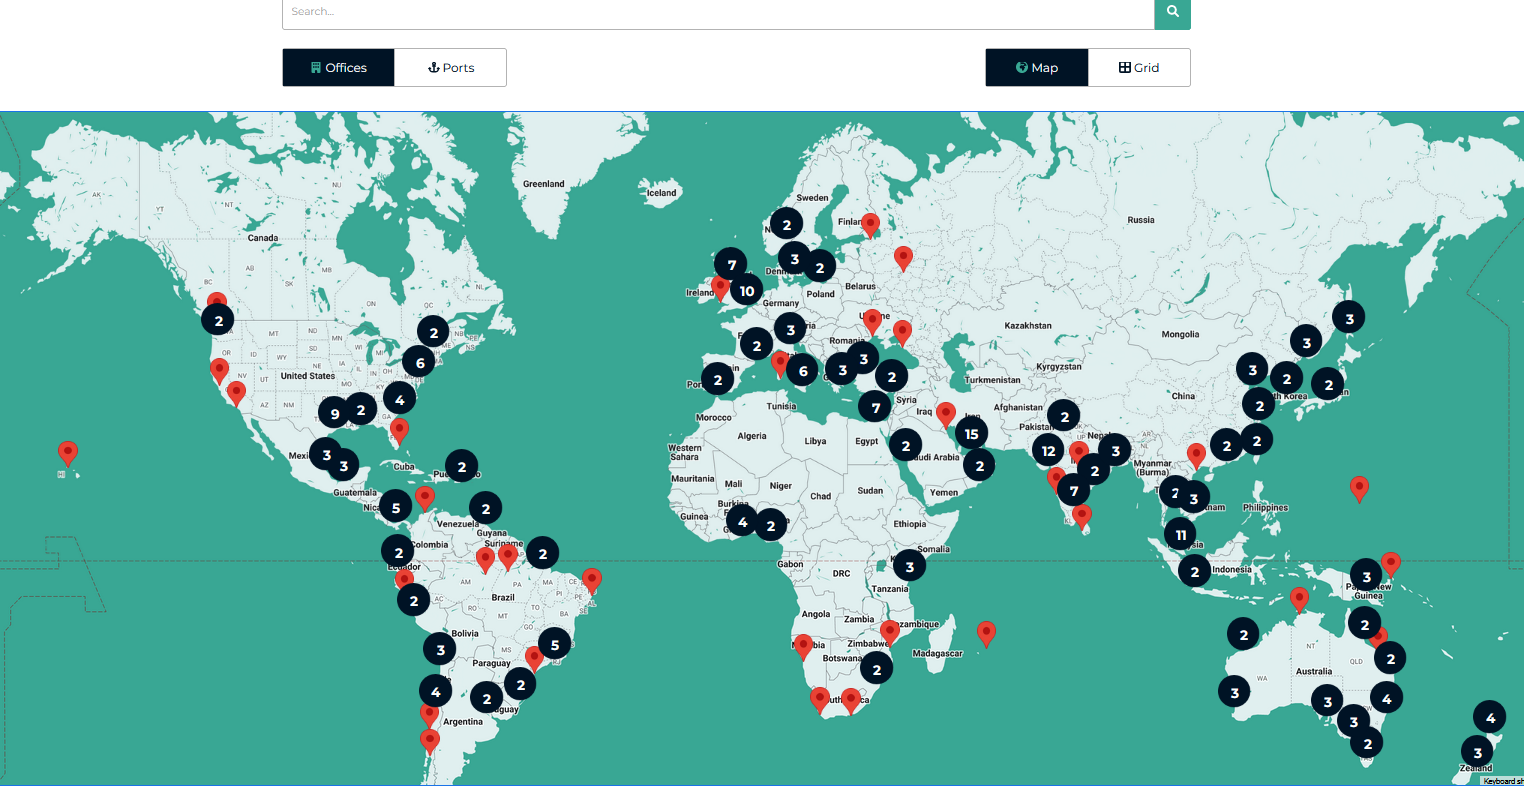
\includegraphics[width=0.5\linewidth]{network.png}
    \caption{From \textit{Inchcape Shipping Services - "Our Network"}}
    \label{fig:Network Map}
\end{figure}
\newpage
\section{Risk Assessment}


\definecolor{adaee4ed-88c8-5b21-a9e7-31316ebef86f}{RGB}{255, 179, 178}
\definecolor{f3551e38-74df-57e2-b793-83d7fe876c85}{RGB}{0, 0, 0}
\definecolor{0b71a967-1f15-55a5-9bb9-70efa7b4fc58}{RGB}{51, 51, 51}
\definecolor{70af333d-4869-5f2a-97ca-9904a9fce6c3}{RGB}{179, 254, 174}
\definecolor{747aec21-333b-59ee-84e3-ddff893e5ccd}{RGB}{255, 216, 176}
\definecolor{5856d031-3da1-575c-834e-c77e9e438c62}{RGB}{162, 177, 195}

\tikzstyle{512bdd77-c3aa-5669-a956-85f7a90c6fb4} = [rectangle, rounded corners, minimum width=3cm, minimum height=1cm, text centered, font=\normalsize, color=0b71a967-1f15-55a5-9bb9-70efa7b4fc58, draw=f3551e38-74df-57e2-b793-83d7fe876c85, line width=1, fill=adaee4ed-88c8-5b21-a9e7-31316ebef86f]
\tikzstyle{b0e005f8-e267-5a3a-a638-881fb9faed1d} = [diamond, minimum width=3cm, minimum height=2cm, text centered, font=\normalsize, color=0b71a967-1f15-55a5-9bb9-70efa7b4fc58, draw=f3551e38-74df-57e2-b793-83d7fe876c85, line width=1, fill=70af333d-4869-5f2a-97ca-9904a9fce6c3]
\tikzstyle{69bbb168-da59-5865-902f-94e77902bf95} = [rectangle, minimum width=3cm, minimum height=1cm, text centered, font=\normalsize, color=0b71a967-1f15-55a5-9bb9-70efa7b4fc58, draw=f3551e38-74df-57e2-b793-83d7fe876c85, line width=1, fill=747aec21-333b-59ee-84e3-ddff893e5ccd]
\tikzstyle{7be24b85-97d0-5b76-ba9e-d94005dca8f2} = [thick, draw=5856d031-3da1-575c-834e-c77e9e438c62, line width=2, ->, >=stealth]
\begin{figure}[hb]

\begin{tikzpicture}[node distance=3cm]
\node (a57c6caf-49dc-4cb6-af62-3cb6fbbe7cad) [512bdd77-c3aa-5669-a956-85f7a90c6fb4] {Gain Access};
\node (0f84e2ea-2de9-4ad6-8522-ff9b9b25b531) [b0e005f8-e267-5a3a-a638-881fb9faed1d, below of=a57c6caf-49dc-4cb6-af62-3cb6fbbe7cad, yshift=-0.5cm] {Physical};
\node (84367632-e919-4a42-8ee6-fb2f30eb2d0c) [b0e005f8-e267-5a3a-a638-881fb9faed1d, right of=0f84e2ea-2de9-4ad6-8522-ff9b9b25b531, xshift=2cm] {Digital};
\node (bcc7fbfc-ce8e-4f39-902d-d726538068ff) [b0e005f8-e267-5a3a-a638-881fb9faed1d, below of=0f84e2ea-2de9-4ad6-8522-ff9b9b25b531, yshift=-0.5cm] {Get Data};
\node (6a5989e1-b4e0-4ed0-8358-6a51e94fb842) [b0e005f8-e267-5a3a-a638-881fb9faed1d, right of=bcc7fbfc-ce8e-4f39-902d-d726538068ff, xshift=2cm] {Cover Tracks};
\node (b652866e-da41-4fed-a7b5-ff3e3c6380ed) [b0e005f8-e267-5a3a-a638-881fb9faed1d, left of=bcc7fbfc-ce8e-4f39-902d-d726538068ff, xshift=-2cm] {Ransom, Sale};
\node (e57a207e-b96f-48db-89c4-8358910a4fc9) [69bbb168-da59-5865-902f-94e77902bf95, below of=bcc7fbfc-ce8e-4f39-902d-d726538068ff, yshift=-0.5cm] {Exfiltrate Data};
\node (3a16c4fd-7489-44c6-b09d-6b1c7084eada) [69bbb168-da59-5865-902f-94e77902bf95, below of=e57a207e-b96f-48db-89c4-8358910a4fc9] {Money};
\draw [7be24b85-97d0-5b76-ba9e-d94005dca8f2] (0f84e2ea-2de9-4ad6-8522-ff9b9b25b531) --  (bcc7fbfc-ce8e-4f39-902d-d726538068ff);
\draw [7be24b85-97d0-5b76-ba9e-d94005dca8f2] (84367632-e919-4a42-8ee6-fb2f30eb2d0c) --  (bcc7fbfc-ce8e-4f39-902d-d726538068ff);
\draw [7be24b85-97d0-5b76-ba9e-d94005dca8f2] (bcc7fbfc-ce8e-4f39-902d-d726538068ff) --  (b652866e-da41-4fed-a7b5-ff3e3c6380ed);
\draw [7be24b85-97d0-5b76-ba9e-d94005dca8f2] (b652866e-da41-4fed-a7b5-ff3e3c6380ed) --  (3a16c4fd-7489-44c6-b09d-6b1c7084eada);
\draw [7be24b85-97d0-5b76-ba9e-d94005dca8f2] (bcc7fbfc-ce8e-4f39-902d-d726538068ff) --  (e57a207e-b96f-48db-89c4-8358910a4fc9);
\draw [7be24b85-97d0-5b76-ba9e-d94005dca8f2] (e57a207e-b96f-48db-89c4-8358910a4fc9) --  (6a5989e1-b4e0-4ed0-8358-6a51e94fb842);
\draw [7be24b85-97d0-5b76-ba9e-d94005dca8f2] (6a5989e1-b4e0-4ed0-8358-6a51e94fb842) --  (bcc7fbfc-ce8e-4f39-902d-d726538068ff);
\draw [7be24b85-97d0-5b76-ba9e-d94005dca8f2] (a57c6caf-49dc-4cb6-af62-3cb6fbbe7cad) --  (0f84e2ea-2de9-4ad6-8522-ff9b9b25b531);
\draw [7be24b85-97d0-5b76-ba9e-d94005dca8f2] (a57c6caf-49dc-4cb6-af62-3cb6fbbe7cad) --  (84367632-e919-4a42-8ee6-fb2f30eb2d0c);

\end{tikzpicture}
\caption[Sample Flowchart]{A flowchart of attacker decisions\protect\footnotemark.}
\end{figure}
\footnotetext{This model does not show specific means of attack, nor include end outcomes like sabotage or defamation. Attackers choose one or more means of ingress, such as an SQL injection or phishing or bogus password reset, get the data that Inchcape needs for work and that governments and black market buyers want, and try to get out without getting caught by defenders.}

 The overall strategic goal of the attackers is also indicative of their likelihood to use a particular strategy. Table \ref{tab:Threat Matrix} shows this broken down by what attackers are likely to use which attacks. 
% Table generated by Excel2LaTeX from sheet 'Sheet1'
\begin{table}%[hbp]
  \centering
  \caption{Color Coded and Numerical table for the likelihood of each attack being used by each attacker.}
    \begin{tabular}{|c|c|c|c|c|}
    \toprule
    \multicolumn{2}{|c|}{\multirow{2}[4]{*}{Risk Assessment Matrix}} & \multicolumn{3}{c|}{Threat Actors} \\
\cmidrule{3-5}    \multicolumn{2}{|c|}{} & Cyber Criminals & Chinese APTs & Iranian Spies \\
    \midrule
    \multirow{5}[10]{*}{\begin{sideways}Attack\end{sideways}} & Physical/Hybrid & \cellcolor[rgb]{ .694,  .831,  .498}2 & \cellcolor[rgb]{ .694,  .831,  .498}2 & \cellcolor[rgb]{ .388,  .745,  .482}1 \\
\cmidrule{2-5}          & DoS  & \cellcolor[rgb]{ 1,  .922,  .518}3 & \cellcolor[rgb]{ .388,  .745,  .482}1 & \cellcolor[rgb]{ .694,  .831,  .498}2 \\
\cmidrule{2-5}          & Social Media & \cellcolor[rgb]{ .388,  .745,  .482}1 & \cellcolor[rgb]{ 1,  .922,  .518}3 & \cellcolor[rgb]{ .988,  .667,  .471}4 \\
\cmidrule{2-5}          & Phishing & \cellcolor[rgb]{ .973,  .412,  .42}5 & \cellcolor[rgb]{ .973,  .412,  .42}5 & \cellcolor[rgb]{ 1,  .922,  .518}3 \\
\cmidrule{2-5}          & Spyware & \cellcolor[rgb]{ .988,  .667,  .471}4 & \cellcolor[rgb]{ .988,  .667,  .471}4 & \cellcolor[rgb]{ .973,  .412,  .42}5 \\
    \midrule
    Scale & Least Likely & \cellcolor[rgb]{ .388,  .745,  .482}1 & \cellcolor[rgb]{ .973,  .412,  .42}5 & Most Likely \\
    \bottomrule
    \end{tabular}%
  \label{tab:Threat Matrix}%
\end{table}%


\newpage

\begin{table}
    \centering
    \begin{tabular}{|c|c|c|}
    \hline
         &High Severity Attacks& High Effort Attacks \\
         \hline
       Cybercriminals  & No Preference & Not Preferred\\
         \hline
        State Actors & Not Preferred & No Preference\\
         \hline
    \end{tabular}
    \caption{Threat Actors by Attack Style}
    \label{tab:Severity Matrix}
\end{table}
\begin{itemize}
    \item Cybercriminals are focused on extracting money by any means. Zero Day exploits are expensive to perform and may not be compatible with target systems, so gangs will often resort to less sophisticated means of ingress, perhaps at the cost of perfect secrecy. Phishing attacks are versatile and inexpensive; attackers can upload their payloads as attachments or trick employees into giving up data, passwords, or even money.\footnote{Spyware is good for collecting data but to turn data into money they need a black market buyer or to resort to blackmail.} Loud attacks like DDoSing the website, defacing social media profiles, encrypting data, or arson and promising to continue those attacks until the random is paid can make money, but carry increased risk of discovery for the attacker. DDoSing a website and hacking a social media account are low severity attacks which are easy to recover from, but are hard to ignore. Encryption Ransomware has much higher severity, but can be thwarted with backups. The freedom to take more extreme measures to achieve strategic and tactical goals makes cybercriminal gangs a more alarming threat than State Backed actors.
    \item State Actors have a different final goal, in the cases examined in Section \ref{actors}, threat groups focused on exfiltrating data over financial gain and causing harm. When attacking private sector targets, they prefer low severity attacks that reduce the chance that defenders will notice an attack in progress, and they have government money to spend on sophisticated hacking tools to achieve this. Phishing and Spyware, for the reasons listed above, go hand in hand and are common for espionage. Trick one person into clicking an attachment in an email and you get all the data your handlers could ever want, so long as your payload also contains something to conceal the fact that data is getting out at all. These hackers are unlikely to use Social Media except as a vector to reach their true target, some partner company to Inchcape\footnote{Depending on that partner, attackers may choose to take a less subtle approach if they believed that those targets represented a more strategically viable bottleneck. Inchcape is replaceable with other businesses. Ships and Ports can live without us, even though it would be worse, and harder, and slower, but the fact that business can continue without us means we are relatively safe from state backed saboteurs.}. In that vein, ransomware attacks DDoS attacks, defacement, and sabotage also call attention to the actor, which goes counter to their strategy, so these high severity attacks are unlikely. 
\end{itemize}

%\newpage
\section{Recommendations}
To reduce the severity and likelihood of the attacks discussed, the following controls may be implemented.
\begin{enumerate}
    \item Train all employees to recognize signs of phishing and other malicious communication.\footcite{baltic_and_international_maritime_council_guidelines_nodate}
    \item Monitor systems for signs of data exfiltration\footnote{Including volumes of data going out over the internet connection at strange hours to unknown servers} and limit the connectivity of vital systems to the internet and the intranet to limit lateral movement.
    \item Require multi-factor authentication and training for all authorized users of the company's internet presence including social media and the Inchcape website.\footcite{mrakovic_maritime_2019}
    \item Maintain backups to ensure the continuation of business in case attacks interrupt service.
    \item Bolster physical security on the premises and restrict the use of outside USB drives and disks.
\end{enumerate}
Sensible controls can minimize system downtime and damage from attacks, reduce the risk of breach or loss of data, and ensure confidentiality with all business partners.

%\printbibliography
\clearpage
\section*{ChatGPT Statement}
I spoke to Dr. Taiyo Inoue about how he uses ChatGPT and other generative AIs at the Connectfest a couple weeks ago. I am not impressed by its output when writing in the essay mode, so I have been putting completed essays as an input and asking it for feedback, an advanced form of Grammerly that can make my writing sound more businesslike. He recommended using it as a sounding board, so that's what I did in this case. I knew I wanted to do something maritime, but also something out of my comfort zone, Chat helped me narrow it down to ship agents. My friend Maura is one, so I picked her company as the target. I don't know a lot about ship agents, so I asked Chat for his impression of what their attack surface and vulnerabilities might be, considering that ChatGPT can only have a layman's understanding in any subject, then to pretend to be a friend whom I ask questions, and ending with asking for a list of search terms I could use to direct my research. This has helped a little, but I still visited Laurie Borchard in the library to find more sources and for tips in winnowing down the ones I found. I tried using it to improve my outline, but it essentially just made a different version of the assignment instructions. For gits and shiggles, I wanted to see what it would look like if he tried to make a few of those bullets into paragraphs, and the results were absolutely inane drivel. Still wrote my paper out the old fashioned way, Overleaf+Zotero. I probably should have started writing it sooner, but oh well.
\section*{Mini Interview with an employee}
\begin{newchat}
Ready to answer questions.
What information systems would be the worst ones to be damaged by a cyber attack? 
No comment 
Do you think that Inchcape is more at risk of being hacked by criminal gangs or governments and terror cells? 
Criminal gangs, we don't work with the government and terrorist cells don't care about entrance/clearance forms but i can see how the black market could work with/around our services
Do you think that the cyber training provided to employees is adequate? 
\end{newchat}
\begin{newchat}
It raises awareness and trains us lightly. We are protected against minor threats. Major threats do occasionally break through whatever defenses we have but we recover/notice almost immediately therefore reducing threat level
What is the worst case scenario? 
Unsure
Are there any systems or people that you worry could be easily broken or compromised?
No, our security is pretty good as is
Thank you, no more questions.
\end{newchat}
\end{document}          
